\chapterpicture{header_07}
\chapter{Farmaci antistaminici}

L'istamina (ammina della pelle) è un ammina biogena molto diffusa nell'organismo
ed è contenuta nei mastociti dove viene sintetizzata e conservata. La sua
concentrazione è particolarmente elevata (circa 1mg/100gr di tessuto) nella mucosa
intestinale, nella cute e nei polmoni.

Nel 1927 l’istamina venne isolata da tessuti
polmonari e epatici e venne quindi riconosciuta come molecola fisiologica.
E’ nota principalmente per il suo intervento nei fenomeni allergici e di anafilassi.
Viene rilasciata in seguito a reazioni di ipersensibilità e in seguito a danni cellulari.
E’ definita un  ``ormone locale'' o autacoide.

L'istamina interagisce con diversi recettori, detti istaminergici. I
recettori sono classificati con dei numeri, quindi si hanno i recettori H\ped{1}, H\ped{2}, H\ped{3} e H\ped{4}.

\fullpicture*{16_001}{Struttura dei recettori istaminergici}

Il recettore H\ped{1} è responsabile delle reazioni allergiche, mentre i
recettori H\ped{2} sono collegati alla secrezioni acide. I farmaci sono
definiti antiulcera.

Per quanto riguarda gli H\ped{3} e H\ped{4}, non si sa molto. Ci sono delle ricerche
in atto. I recettori H\ped{3} sono stati scoperti nel 2000, quindi è molto
difficile avere un farmaco nel breve (20 anni) periodo.

I recettori H\ped{1} e H\ped{2} sono stati scoperti nei primi anni del 900. In quel
periodo i farmaci erano sviluppati con il metodo \emph{trial and error}.

Quindi alcuni farmaci erano in grado di inibire entrambi i recettori,
mentre altri sono uno dei due. Quindi si è ipotizzata l'esistenza dei
due recettori. I farmaci sono stati sviluppati senza sapere la struttura
del bersaglio.

\section{Istamina}

L'istamina ha una catena alifatica. Si ha un carbonio \alpha{} e uno
\beta. È possibile avere una tautomeria.
L'azoto \pi{} è quello più vicino alla catena, mentre l'azoto più
distante è quello \tau.
I due tautomeri prendono il nome da questi due azoti.
\begin{figure}[H]
  \centering
  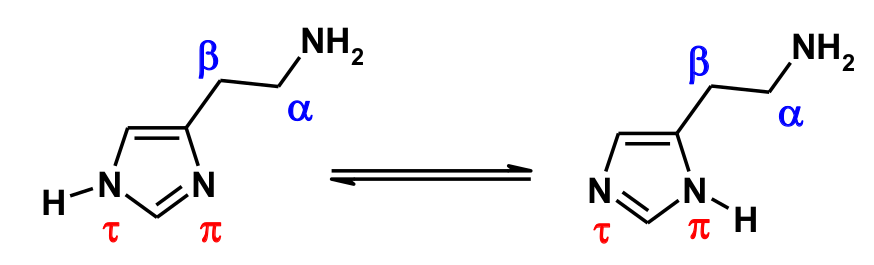
\includegraphics[width=\textwidth]{16_002}
\end{figure}

L'istamina è presente nella pelle, da cui prende il nome. Si trova nella
mucosa intestinale e nei polmoni oltre che sulla pelle e anche sulla mucosa
gastrica.

Infatti le reazioni allergiche avvengono prevalentemente a livello
polmonare (respiratorio) e cutaneo.

L'istamina si trova all'interno dei mastociti, che sono cellule
immunitarie, e questi sono presenti all'interno di questi tessuti.

Iniziando a parlare di antistaminici (recettori H\ped{1}), si collegano gli
antistaminici a questo recettore, però si deve ricordare che ha anche un
altro target. Essendo un neurotrasmettitore, va anche a interagire con
il SNC.

L'istamina viene conservata come riserva, all'interno dei mastociti. Il
livello nel sangue è molto basso.
L'istamina viene riconosciuta come ormone locale, perché viene
rilasciata in modo locale. L'emivita è molto breve, però la risposta è
molto forte, perché l'istamina viene rilasciata in grande quantità.
I due tautomeri possono essere presenti anche nelle due forme ionizzate.

A ph 7.5, l'istamina si trova nella forma protonata, a livello dell'azoto alifatico.
La forma bicarica può esistere, però questo avviene in una percentuale
molto bassa (a ph fisiologico), però questo può essere rilevante ad un
pH gastrico.

Bisogna considerare questi equilibri in base a dove l'istamina si trova.
Il rapporto tra i due tautomeri (i valori sono delle ipotesi), la forma
protonata in \tau{} è preponderante a quella in \pi, con un rapporto di 4:1.
Per fare questo rapporto, si è utilizzato un radiotracciante.

\clearpage

\begin{figure}[H]
  \centering
  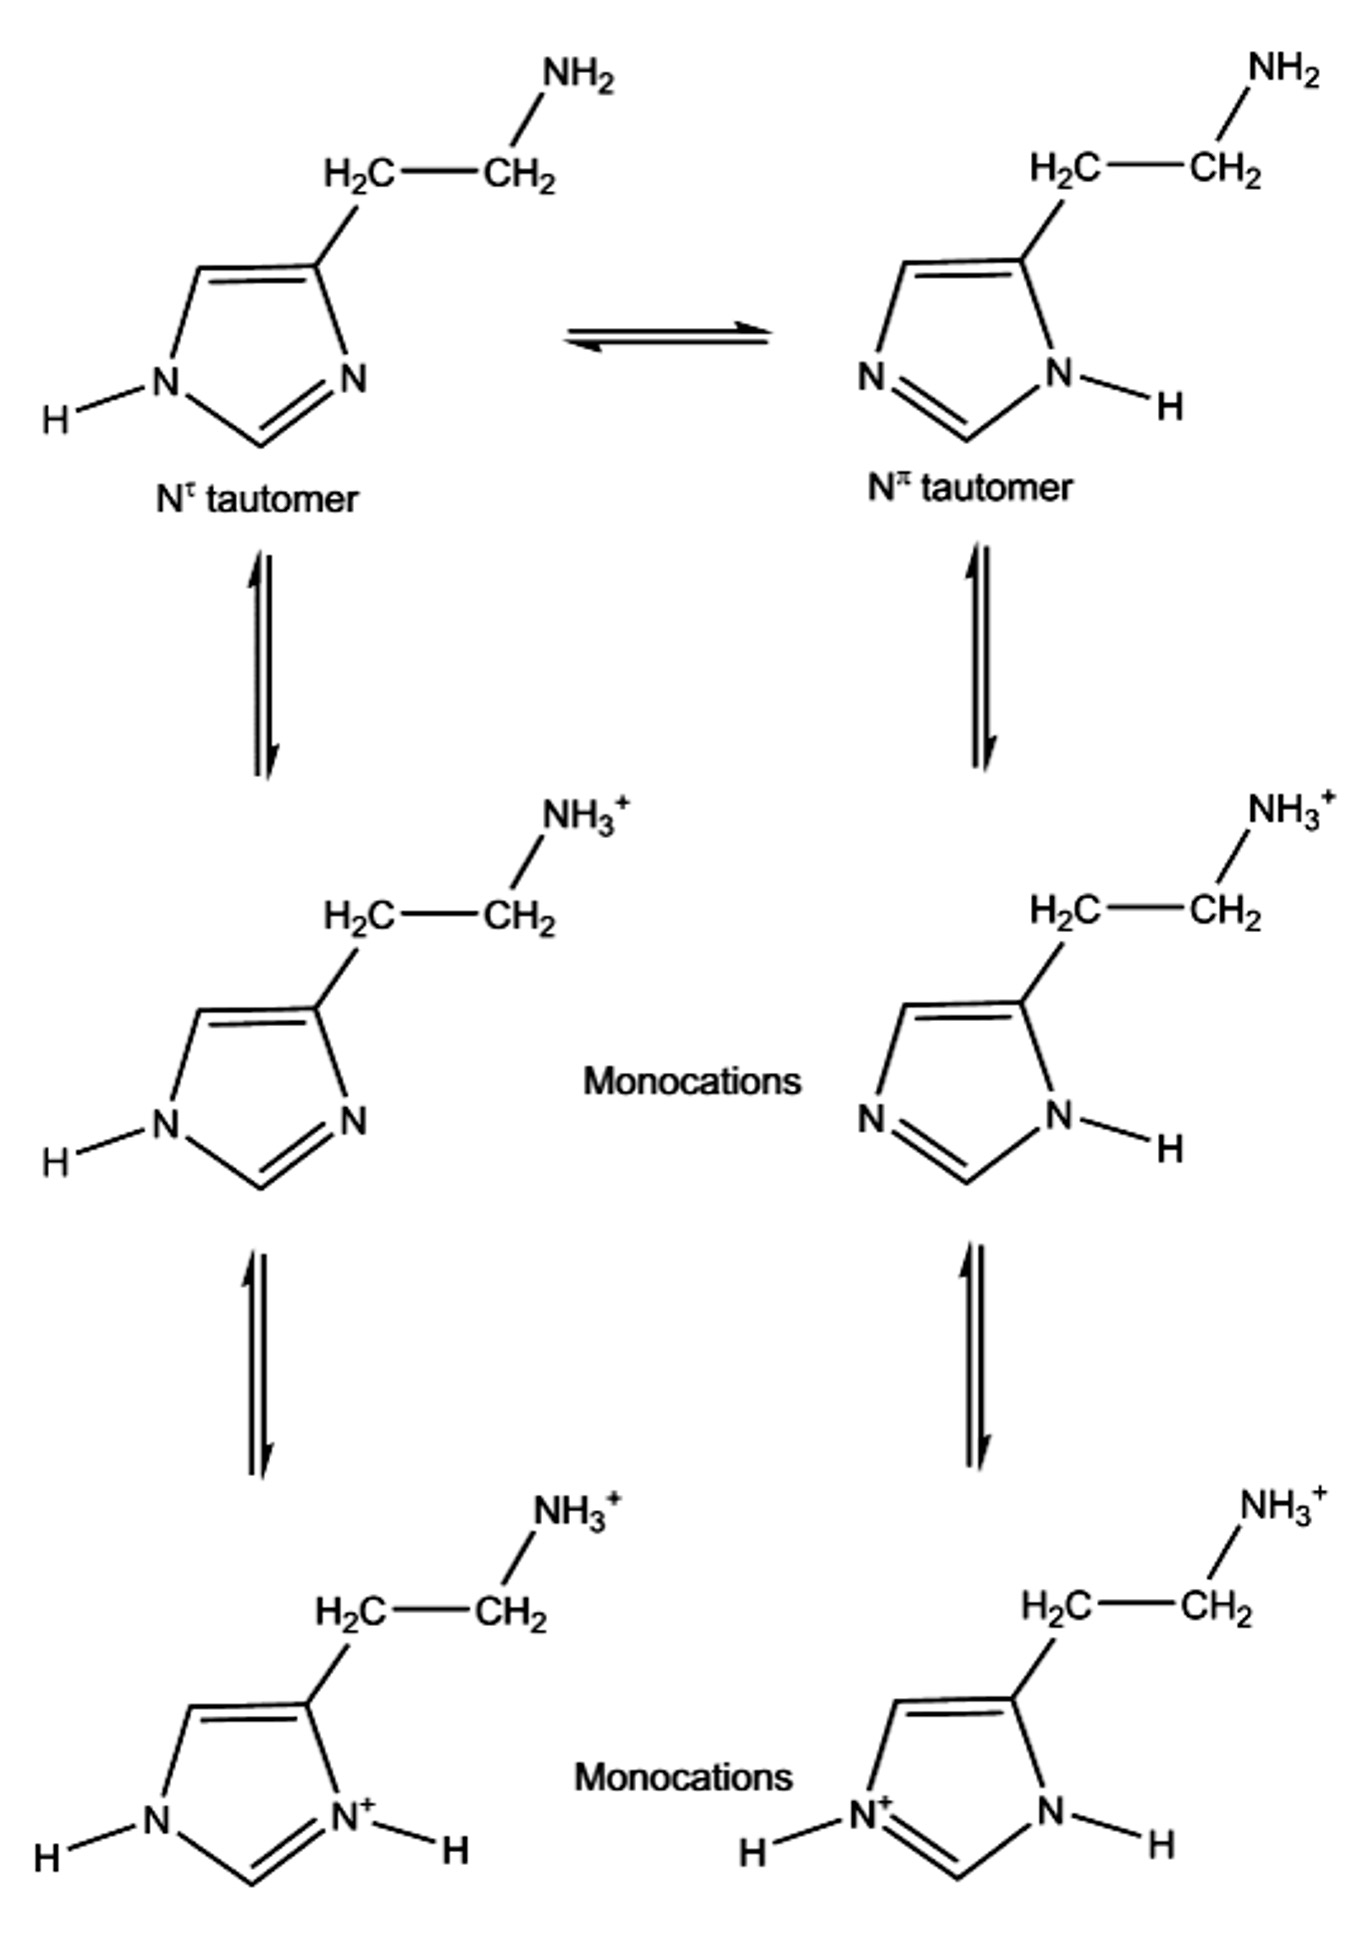
\includegraphics[width=0.5\textwidth]{16_004}
\end{figure}


L'istamina è una molecola che viene prodotta dall'organismo; la
biosintesi parte dall'istidina, grazie ad alcuni enzimi. Avviene una
decarbossilazione dell'istidina.
L'istamina viene sintetizzata e accumulata.
\begin{figure}[H]
  \centering
  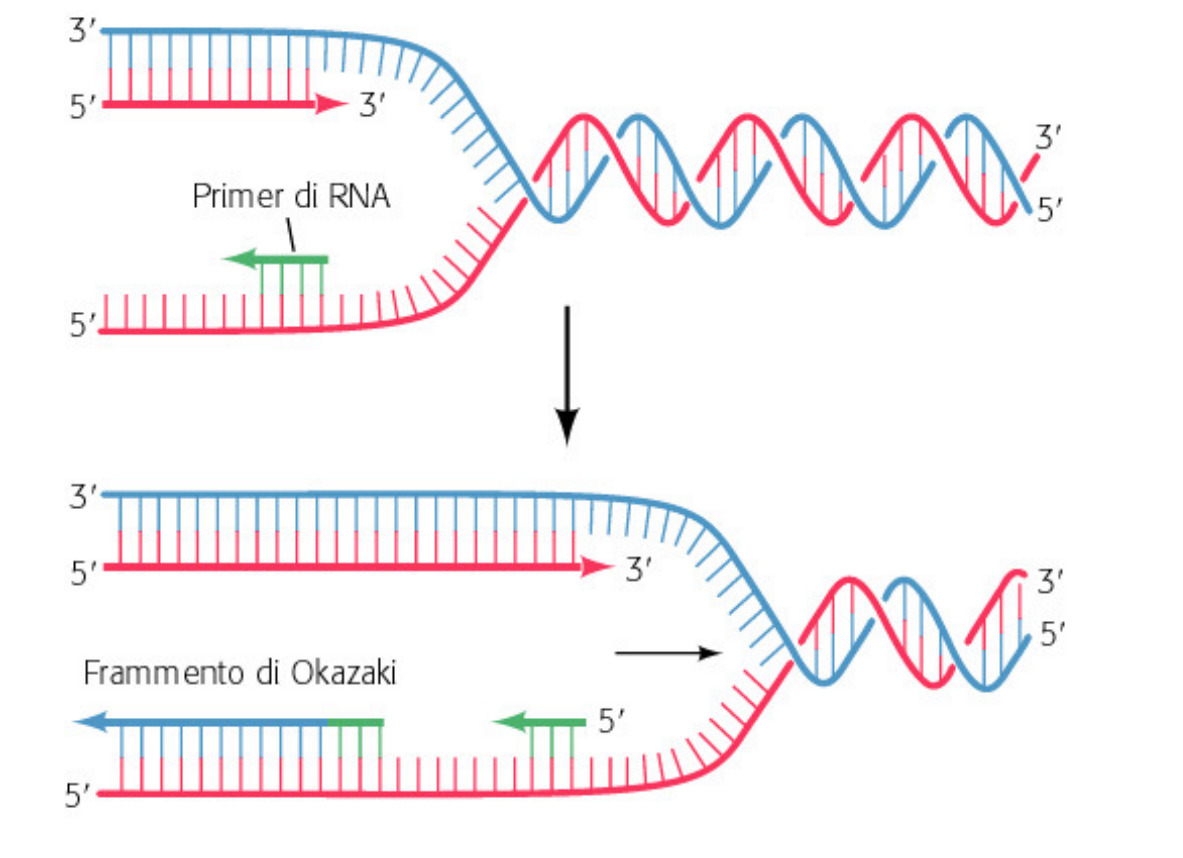
\includegraphics[width=\textwidth]{16_003}
\end{figure}


La capacità dell'istidina di poter essere liberata localmente presuppone
che il metabolismo sia veloce.
In primis, il meccanismo è la metilazione dell'azoto in tau.
Un ulteriore passaggio (due) è un'ossidazione.
Poi la molecola può essere eliminata.
Gli enzimi utilizzati sono ossidasi o metilasi
\begin{figure}[H]
  \centering
  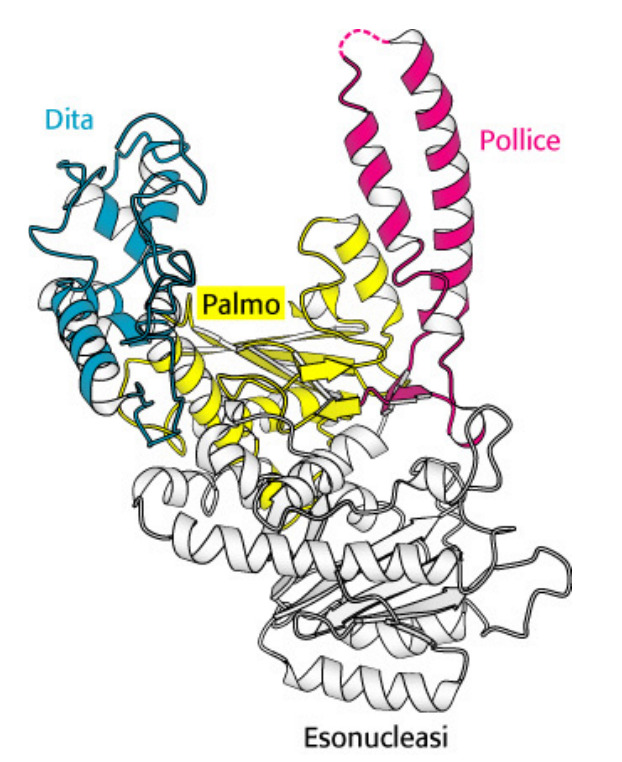
\includegraphics[width=\textwidth]{16_005}
\end{figure}

In alternativa a questo pathway, l'istamina viene ossidata e poi
attaccata da un gruppo ribosil. Questo pattern non è comune, però per
l'istamina è una via possibile.

Le proprietà dell'istamina sono:
\begin{itemize}
    \item Reazioni allergiche 
    \item Reazioni infiammatorie
    \item Secrezione acida
    \item Neurotrasmettitore
\end{itemize}

Le infiammazioni sono strettamente collegate alle reazioni allergiche.

I tessuti dove è presente l'istamina sono molto estesi, basti pensare
alla cute o all'intestino. La molecola può essere definita ubiquitaria,
ovvero presente ovunque.
Gli altri tessuti sono ricchi di mastociti (dove viene sintetizzata e
accumulata). L'istamina viene anche sintetizzata e accumulata nelle
sinapsi (nell'SNC).
All'interno delle cellule, ci sono dei grani, che accumulano l'istamina.
Mentre nei neuroni viene contenuta all'interno di vescicole sinaptiche.
Quando è il momento di rilasciare, causa la risposta allergica.

Al momento del rilascio neuronale, l'istamina viene rilasciata a seguito
di un segnale. Mentre a livello di altri tessuti, avviene un
riconoscimento tra antigene e anticorpo. I mastociti, dopo essere stati
esposti, sviluppano delle immunoglobuline sulla superficie. Quando
l'anticorpo ritrova l'antigene, allora viene rilasciata l'istamina.
(Utilizza dei canali del \ce{Ca^{2+}})
Questo processo viene definito ``degranulazione dei mastociti''. Quindi,
si ha una risposta allergica.

\fullpicture*{16_006}{Ruolo dei mastociti nell’infiammazione}

Si vede l'antigene-anticorpo, che consente la liberazione di istamina,
ma anche di altri neutros spettatori che sono coinvolti nella risposta
infiammatoria.
Per semplicità si guarda solo l'istamina, però in realtà la situazione è
molto più complessa, in quanto avvengono più eventi di quello che sembra.

\marginbox{Puntura d'ape}{
Dalla prima volta che si viene in contatto con un antigene, non si hanno
ancora gli anticorpi. La prima volta non è letale, ma la seconda
potenzialmente lo è. La reazione che si innesca può essere molto più grave
e molto più veloce. L'evoluzione della risposta allergica può essere
vista nello schema del mastocita.
Si ha quindi una sensibilizzazione all'antigene.
}

A livello della sinapsi invece, avviene una cosa diversa.
In questa rappresentazione, si vede schematizzata una sinapsi. Nella
sinapsi ci sono diversi recettori istaminergici.
Il recettore H\ped{1} è molto più presente a livello dei neuroni.

\fullpicture*{16_007}{Recettori instaminergici presenti nelle sinapsi}

All'interno del neurone sono presenti le vescicole. Quando il calcio
varia, l'istamina viene rilasciata. In parte viene metabolizzata e in
parte reagisce con i recettori che trova.

Se l'istamina va verso il recettore sinaptico si prevede la reazione
desiderata.

I recettori H\ped{3} invece fungono da autorecettori, quindi l'istamina va a
interagire con il neurone stesso, in modo tale da regolare l'istamina
all'interno del secondo neurone.

Nel SNC, sono presenti anche gli H\ped{1}, in quanto l'istamina viene
utilizzata per regolare una ulteriore risposta a livello di altri
messaggeri. Questo è il segnale responsabile del rapporto sonno/veglia.
Questo è un effetto collaterale, in quanto quando si prende un
antistaminico si ha sonnolenza. Questo è un effetto collaterale in
quanto non si vuole avere sonnolenza.

Questo è per far capire che un farmaco interagisce con più bersagli, o
con lo stesso bersaglio, che però produce un effetto diverso.

Le sigle dei quattro recettori sono
\begin{itemize}
  \item \emph{H\ped{1}R:} Histamine 1 Receptor
  \item \emph{H\ped{2}R:} Histamine 2 Receptor
  \item \emph{H\ped{3}R:} Histamine 3 Receptor
  \item \emph{H\ped{4}R:} Histamine 4 Receptor
\end{itemize}

\marginpicture*{16_008}{Struttura del recettore H\ped{1} complessato con dossepina}

I recettori vengono definiti recettori di superficie.

Un effetto collaterale degli antistaminici può essere anche la
depressione.

Guardando la struttura dei recettori H\ped{1}, si vede che questa struttura è
associata alla struttura G, che ha un modo particolare di reagire.

\fullpicture*{16_009}{Classificazione dei recettori instaminergici con le loro attività. }

I recettori a livello dell'organismo sono classificati in diverse
classi.
Hanno un'azione diversa, a livello di effetto e di pathway di reazione.
I recettori accoppiati alla proteina G convertono il GTP in GDP.

\fullpicture*{16_010}{Recettori instaminergici accoppiati alla proteina G.}

Come tutti i recettori, c'è bisogno di un agonista che interagisca con
il recettore. Questo recettore si trova transmembrana, si hanno quindi
due sovrapposizioni con lo spazio extracellulare e intracellulare.
L'agonista in questo caso è l'istamina, che attiva una proteina G.
La proteina G poi rilascia un cofattore, che funge da secondo
messaggero, che può essere ipoespresso o iperespresso.
Si ha l'attivazione di un segnale.

Questi recettori hanno una struttura ben definita. (così come altri
recettori, come quelli muscarinici). Hanno una sequenza diversa, però.

Sono presenti sette eliche, connesse tra vari loop.

C terminale, spazio intracellulare. N terminale, spazio extracellulare.

Dalla struttura vista prima, sono presenti sette eliche.

Questo recettore, quando inattivo, ha una conformazione più estesa. Però
quando l'agonista si lega, il recettore cambia conformazione e si
restringe.

Tutti i recettori H simili a livello di struttura e di meccanismo.

Il terzo loop nello spazio intracellulare è responsabile
dell'attivazione della proteina G. L'attivazione della proteina G porta
all'attivazione del messaggero secondario, (che cambierà a seconda del
recettore).

Il fatto che ci sia l'attività GTPasica, comporta il processo di avere
un secondo messaggero.

Nel caso dei recettori istaminergici, si hanno diversi messaggeri:
\begin{itemize}
    \item H\ped{1} IP3 (Inositolo trifosfato) 
    \item H\ped{2} cAMP (Adenosina Monofosfato Ciclica)
\end{itemize}

Ogni messaggero comporterà un effetto finale diverso.

I recettori H\ped{3} sono più presenti a livello di SNC, e sono in grado di
comandare un secondo neurone, il rilascio di dopamina. Il sistema
autorecettore, causa il controllo della sintesi e del rilascio di
dopamina.

Gli antagonisti H\ped{3}, sono in grado di superare la barriera
ematoencefalica e sono implicati anche nel mantenere il ritmo sonno
veglia e sono dei soppressori dell'appetito.

L'ordine della localizzazione è in base alla quantità presente negli
organi. Ad esempio, H\ped{1} si trova nella muscolatura liscia nella
maggioranza dei casi. Si ha anche l'effetto di tachicardia.

La contrazione della muscolatura liscia può significare asma (azione) o
arrossatura a livello della cute.
Si prende un antistaminico se si ha una risposta allergica.

I recettori H\ped{2} sono responsabili della secrezione gastrica. SI trovano
anche in altri organi importanti, quindi possono avere degli altri
effetti, spesso collaterali.
Ad esempio, una risposta allergica può determinare la contrazione della
muscolatura liscia (utero), che può determinare anche un aborto.

\marginbox*{
Se si conoscono le macchine molecolari (target), si possono sviluppare
dei farmaci che abbiano degli effetti collaterali meno intensi.
}

I recettori H\ped{4} sono ancora meno conosciuti, si trovano nel midollo osseo
e nella milza.

La proteina G non è una sola proteina, ma una classe di proteine, quindi
le attivazioni sono specifiche.
La reazione allergica avviene quando anticorpo e antigene vengono a
contatto; si libera istamina.

La risposta che avviene è triplice 
\begin{itemize}
  \item \emph{Rossore:} dovuto alla dilatazione
  dei capillari 
  \item \emph{Gonfiore:} dovuta da una aumentata permeabilità della
  zona; si ha un edema 
  \item \emph{dolore:} l'istamina può anche influire sui nervi,
  quindi si ha una sensazione di dolore (prurito).
\end{itemize}
L'istamina va a contrarre la muscolatura liscia, con conseguenti effetti
nefasti.

\fullpicture*{16_011}{Tabella dei recettori instaminergici}

Gli effetti dovuti alla risposta istaminergica, avvengono anche a
livello cardiocircolatorio. Questo può provocare aritmie/tachicardia; si
aumenta la velocità (frequenza) e della potenza cardiaca. Questo può
provocare un aumento della pressione sanguigna.
Se si lavora con questi recettori, possono esserci effetti collaterali,
anche a livello cardiaco. Questi effetti si è cercato di ridurli.

L'istamina si comporta da autacoide, viene rilasciata a livello locale e
ha un metabolismo molto veloce. Provoca la vasocostrizione (a livello di
bronchi), anche a livello oculare (prurito agli occhi).

Si vedono dei farmaci che ora sono stati utilizzati, tanto tempo fa. Non
funzionavano come antagonisti dei recettori H\ped{1}. L'effetto è quello di
antagonista, anche se in realtà sono degli agonisti inversi.

Un agonista inverso agisce sempre come antagonista; l'antagonista lega
sia la forma attiva sia la passiva, mentre l'agonista inverso lega solo
la forma passiva

L'istamina una volta legata cambia conformazione. Gli antistaminici si
legano alla forma inattiva e non permette l'effetto a cascata causato dall'istamina.

\fullpicture{16_012}{Tabella degli agonisti. Non si utilizza il nome commerciale, ma il nome del principio attivo. $+$ Effetto molto attivo $-$ effetto meno attivo.}{tab:insta}

Come si vede nell'imamgine \ref{tab:insta}, sono presenti gli antistaminici di prima generazione e di seconda generazione.
La differenza è molto intuitiva, i farmaci di seconda generazione sono
l'evoluzione dei farmaci di prima generazione. Quelli di prima
generazione, hanno degli effetti collaterali importanti; se si riesce ad
eliminare l'effetto collaterale, il farmaco diventa di seconda
generazione. Si basa anche su una scala temporale.
Per ciascun farmaco viene classificato con una serie negativa o
positiva. 

I farmaci di prima generazione sono efficaci con il recettore H\ped{1}.
Hanno un'azione sedativa in quanto i settori H\ped{1} sono presenti nei
neuroni, per il ciclo veglia-sonno.

\marginbox*{
Un altro recettore è quello muscarinico, su cui questi farmaci hanno un
attività. I recettori muscarinici sono molto simili ai recettori H e
quindi è difficile avere selettività per i recettori H rispetto a quelli
muscarinici.\\
Questi farmaci possono avere un'attività che causa depressione, in
quanto i recettori muscarinici determinano l'azione della serotonina.
}

Fino alla prima generazione, si ha una forte attività istaminica, ma
anche una forte attività sedativa e una attività come antimuscarinici.
Questo comporta che gli effetti collaterali erano molto elevati.
In seguito, si è cercato di avere una certa selettività. Gli
antistaminici di seconda generazione sono molto più selettivi.

Questo non significa che si utilizzano solo i farmaci di seconda
generazione, ma anche quelli di prima generazione, a seconda del
soggetto e della situazione (es. graminacee o altro). La componente
individuale è molto importante.

La maggior parte dei farmaci non presenta effetti antiemetici, però
alcuni si; questo consente di contrastare gli effetti di nausea dovuti al mal di
mare e vi sono delle gomme da masticare, dette travel-gum, che contengono queste molecole.
I farmaci che presentano questo effetto possono essere utilizzati come antistaminici.
Data la struttura della molecola del travel-gum, si vede che la forma
cloridrato ha effetto collaterali maggiori; non può essere assunto come
pillola, ma deve essere masticato.

\marginpicture*{16_013}{Dimenidrinato. La struttura ricorda la parte alifatica dell'istamina; gli antagonisti
prendono spunto dall'agonista, in modo tale da competere con l'istamina.}

\section{\texorpdfstring{Antagonisti dei recettori H\ped{1}}{Antagonisti dei recettori H1}}

Le caratteristiche sono proprie dei farmaci di prima generazione. Si
prende questo come esempio per vedere lo sviluppo del farmaco.
Sono antagonisti dell'istamina e sono inibitori reversibili, quindi il legame non è covalente.

La struttura ricorda quella dell'istamina, non c'è un anello di
imidazolo, ma presentano lo stesso degli anelli aromatici. Un'ammina
alifatica viene mantenuta e il linker sarà composto da due/tre atomi di
carbonio.
C'è anche un atomo a ponte tra i due aromatici.

I farmaci di prima generazione hanno un effetto intenso sul SNC, con i
relativi effetti collaterali.

\subsection{Prima generazione}

Si hanno due gruppi aromatici. In base all'atomo a ponte si chiama il
farmaco. Si hanno anche due o tre atomi di carbonio legati all'ammina
terminale, che può essere alchilata.

Queste sono delle SAR di base, non è che tutti i farmaci visti avranno
questa struttura, alcuni possono averla diversa.

I farmaci di prima generazione agiscono a livello dell'SNC. Gli effetti
collaterali possono essere stimolati, ma anche effetti deprimenti
dell'SNC. Questi effetti possono essere presenti a seconda della
variabilità del paziente.

I farmaci utilizzati in precedenza non ricordano la struttura vista in
precedenza. Sono stati utilizzati per partire a sviluppare altri
farmaci. \marginpicture*{16_016}{Kellina} \marginpicture*{16_017}{Cromolina}
Ad esempio, la cromolina non è un vero e proprio antistaminico
(antagonista). Agisce invece a livello del rilascio dei granuli
dell'istamina. Questo è un possibile meccanismo di reazione, però non è
stato perseguito. Quindi si impedisce la degradazione dei mastociti.

\marginpicture*{16_015}{Piperossano}

Da queste strutture deriva il primo antagonista, ovvero il \emph{piperossano}.
Questo farmaco non è più utilizzato, e la sua struttura non è stata più
utilizzata per gli effetti collaterali intensi, a carico del sistema
circolatorio.
Su questo farmaco non sono stati fatti studi sull'enantiomeria.

\marginpicture{16_014}{SAR degli farmaci antistaminici di prima generazione}{fig:SARAntistaminiciI}

Il lavoro che è stato fatto è fatto a partire dalla struttura
dell'istamina: le caratteristiche farmacoforiche sono quelle descritte
dalla figura \ref{fig:SARAntistaminiciI}.

Quando l'atomo a ponte è l'azoto, si avranno le classi delle etilammine o
delle etilendiammine. Gli esempi visti sono i farmaci più noti e più
importanti per ogni categoria.

La tonzilamina viene utilizzata per gli stati infiammatori a carico
dell'occhio, si aumenta la lacrimazione.
Un analogo di seconda generazione è l'antazolina. La separazione tra i due
azoti viene mantenuta, però si sostituisce le ammine primarie con
l'imidazolo.

\herepicture{16_018}{0.8}

Quando l'atomo a ponte è invece un carbonio, si parla dei derivati
propilamminici.

Un esempio è la feniramina. Le due funzioni aromatiche possono essere
funzionalizzate ulteriormente. Questo farmaco è utilizzato come
collirio.

A questa sottoclasse appartiene anche la clorfenamina; l'unica
differenza con quella prima è l'aggiunta di cloro.
Il cloro aumenta la potenza e la durata del farmaco. Gli stati
patologici per i quali è utilizzata sono diversi.
In questo caso c'è un centro chirale.
A partire da questo, si separa l'e
nantiomero S, che prende il nome di
desclorfeniramina. Il farmaco si chiama polaramin, che indica che uno
dei due stereoisomeri è attivo (polar).

\herepicture{16_019}{0.8}

\clearpage

Un'altra categoria è quella degli amminoalchil eteri. È stata introdotta
il gruppo etereo.

\herepicture{16_020}{0.8}

Dal punto di vista delle SAR, questo gruppo è importante, in quanto
questi farmaci hanno degli effetti collaterali di tipo colinergico, che
causano secchezza della bocca, visione sfuocata, tachicardia.

Una cosa interessante è che modificando uno degli anelli aromatici,
questo determina una selettività diversa per i recettori colinergici o
istaminergici.
Sostituendo l'idrogeno con il Me, con Et o un t-Bu, in para, si aumenta
l'attività antistaminica.
Se invece si sostituisce in posizione 2, si ottiene l'effetto opposto.
Questo è dovuto ad un blocco conformazionale, questo determina anche lo
sviluppo di farmaci per altre patologie. Questo farmaco viene utilizzato
per il parkinson.

\marginbox*{
Una piccola modifica comporta che il farmaco possa essere utilizzato per
patologie diverse.
}

Sempre per la famiglia degli alchileteri, si vede che viene introdotto
un metile nel centro sterico, che comporta la formazione di una
specifica conformazione della molecola. Questo viene utilizzato come
antinfiammatorio (doxilamina).
Un farmaco di seconda generazione (ebastina), questo farmaco è un
farmaco più rigido, in quanto si ha un anello al posto di una catena.

\herepicture{16_021}{0.8}

Ci sono delle altre strutture che non fanno parte delle classi chimiche
viste fino ad ora, sono altrettanto attivi e usati come antistaminici.

Nell'epinastina si ha un tricliclo con una simmetria ben definita.
Questo per introdurre in gruppo farmacoforo un doppio legame, per dare
più rigidità alla molecola.
Anche la funzione rigida è amminica, che è più rigida di una catena
alifatica.

\herepicture{16_022}{0.8}

Le funzioni aromatiche sono unite da un secondo ponte (ciproeptadina),
queste fanno parte della categoria dei triciclici.
Questo determina una riduzione degli effetti collaterali del SNC; si
cerca di capire la selettività di un farmaco per i recettori H\ped{1} rispetto
ad altri recettori.

\marginbox*{
Le strutture vanno sapute per l'esame, però non bisogna disegnarle dal
nulla. Va anche saputo il nome.
}

In questo sviluppo dei farmaci antistaminici, si è arrivati a dei
farmaci con degli effetti collaterali minori a carico dell'SNC.
Guardando la prometazina, si vede che è in parte un antistaminico, però
è utilizzato come antipsicotico, in quanto l'attività è molto più
intensa per H\ped{1}.

Da un punto di vista strutturale, si può notare che è presente il
sistema triciclico. Un triciclo è planare, mentre l'altro no.
Questo significa che un ciclo planare non va bene per l'attività
antistaminica.
Questi due farmaci sono antagonisti H\ped{1}, però le differenze strutturali
danno la specificità alla molecola.

\herepicture{16_023}{0.8}

Con l'introduzione di queste simmetrie (tricilo bloccato) si ottiene una
certa simmetria nella molecola. In questo caso, con delle sostituzioni
si ottengono degli isomeri costituzionali.
Si vede che è presente l'atropoisomeria, che indica che è presente una
struttura bloccata, che consente di avere due isomeri.
Alcuni studi indicano che questa molecola è più attiva in un isomero,
però (per ora) si utilizza una miscela racemica.
Si usa come sale, per un'azione topica.

\marginbox*{
Si tende ad usare degli isomeri che possono separarsi come solidi
differenti, in quanto rende la separazione molto semplice.
}

Guardando la mizolastina, si vede che la struttura è complessa e rigida,
e l'attività è molto specifica. Ci sono pochi effetti collaterali.

\herepicture{16_024}{0.8}

\subsection{Seconda generazione}

Sono farmaci che sono stati messi in commercio da circa 30 anni. Non
sono nuovissimi, però non c'è interesse nel migliorare una cosa che va
già bene.
Sono chiamati antistaminici selettivi. Hanno una selettività specifica
per il recettore H\ped{1}, non si hanno molti effetti collaterali
Questi farmaci hanno un attività locale, non passano la barriera
ematoencefalica, in quanto sono zwitterioni. Quindi non hanno molti
effetti collaterali dal punto di vista del SNC.

Come esempio si prendano le molecole di fexofenadina e di levocavastina. Sono stati inseriti molti cicli ingombranti, che conferiscono rigidità
alla molecola.

Nella fexofenadina, si vede che il farmaco è il principio attivo, però è un metabolita
di un pro-farmaco, ovvero si assume il profarmaco e una volta
metabolizzato, il farmaco diventa attivo. Un metile del ter-butile viene
ossidato a COOH.
Nella levocavastina, si vede che la molecola è rigida; questo è caratterizzato da un
effetto molto rapido, però con una durata molto elevata.

\herepicture{16_025}{0.8}

Altri farmaci di seconda generazione derivano da quelli di prima.
La struttura è un tricilo. Anche in questo caso, si tratta di un profarmaco (loratadina), mentre il farmaco vero e proprio è la desloratadina.

\herepicture{16_026}{0.8}

Per concludere, si vede la cetirizina, che possiede una stereochimica
(solo l'isomero levogiro è attivo). È utilizzato per sintomi nasali e
oculari locali.

\herepicture{16_027}{0.8}

\subsection{Struttura dei recettori}

Tutti i farmaci sviluppati visti finora sono stati sviluppati senza
sapere la struttura del recettore.
Ad esempio, la dossepina è stata costruita pensando a farla legare con
il recettore H\ped{1}. Viene utilizzata come antidepressivo.

\marginpicture*{16_028}{Recettori istaminergici H\ped{1}}

Ai raggi X, si vede che nel recettore H\ped{1}, c'è una tasca anionica (con
dei residui basici), che si pensa che sia complementare alla porzione
carbossilica dei farmaci di seconda generazione. Questo serve per capire
quanto è importante sapere la struttura del recettore.
Infatti le industrie chimiche investono molto per la struttura
cristallografica della proteina.

La collaborazione tra i vari settori serve per ottenere una struttura.
Servono dei dati per costruire dei modelli, per lavorare in silico con
pochi costi.
Una tecnica nuova è la cryo-em. Questa è una tecnologia nuova, ci sono
pochi centri che hanno la strumentazione necessaria per fare cryo-em.

Si usa la spettrometria di massa per determinare la struttura dei
bersagli molecolari. Questa è una tecnica abbastanza nuova; da sola
questa tecnica non è potente, però associata ad altre tecniche, diventa
molto potente.
Ad esempio, dati degli anticorpi monoclonali, si vuole verificare che
diversi batch siano uguali, o si può studiare la struttura del target

La prima categoria utilizza una piccola molecola (probe), che va a
interagire con il target. Ci sono delle interazioni specifiche.
La piccola molecola va a interagire con dei gruppi amminoacidici esposti
sulla superficie. Una volta eseguita la reazione, quindi con modifiche
covalenti (monoadotto piuttosto che crosslinking) e quindi
irreversibili. Si utilizzano delle proteasi, per tagliare la proteina in
modo specifico. I frammenti vengono analizzati con MS.
Si avranno dei peptidi non modificati (segnati in blu) e poi si avrà una
serie di peptidi modificati dal probe. Quindi si capisce la zona
accessibile al probe (zona superficiale).
In seguito, con altre tecniche, si può risalire alla struttura della
proteina.

Con le altre tecniche, si espone la proteina al deuterio, in seguito
viene bloccata per consentire lo scambio di H con D. Si può parlare di
pochi secondi o di ore.
Le parti possono esposte al solvente scambiano D più velocemente. Questo
consente di avere delle informazioni strutturali.

Infine, ci possono essere degli studi di MS nativa, per verificare che
ci sia interazione non covalente con un probe.

L'integrazione dei dati è fondamentale per la determinazione della
struttura del recettore. Si velocizza quindi l'ottenimento della
struttura del farmaco.

La spettrometria di massa è molto utilizzata, ed è anche molto
importante per la determinazione della struttura del farmaco.

\subsection{NMR e MS}

Si guarda l'applicazione delle tecniche in chimica farmaceutica.
Ad esempio. su uno studio della struttura di alcune proteine, si va a
scrivere il target e le tecniche. Si scrivono anche i risultati attesi e
i risultati ottenuti, quindi presenta anche la conclusione, con una
parte di novità. Bisogna aggiungere una parte che non è stata ottenuta
da altri articoli scientifici.
Ad esempio, nell'articolo visto, si parla dell'acqua nel target. Il
legame non avviene se, per spostare l'acqua di solvatazione, si
necessita troppa energia.

L'NMR necessita di proteine marcate con isotopi Serve una ``grande'' quantità
di proteina (quantità accessibili) Conveniente per proteine piccole
Informazioni su struttura e soluzione Informazioni su regioni
flessibili, protonazione e acqua

La cristallografia necessità di avere dei cristalli Serve una quantità più piccola di
proteina, molto concentrata Conveniente per proteine ben strutturate
Informazioni statiche della proteina
Nella cristallografia si hanno delle soluzioni molto concentrate, maggiori di 10 mg/mL. Però le proteine devono essere insolubili, per
poter cristallizzare. L'elevata concentrazione deve essere in ambiente
organico (DMSO solitamente).

L'NMR ha un limite massimo (30.000 Da), però dà informazioni strutturali
in soluzione e soprattutto dà informazioni sulle regioni (flessibili o
rigide, possibili siti di protonazione e presenza d'acqua).

Queste tecniche sono entrambe utili, mentre i contro servono per
decidere quali e come usare i dati. Può essere che proteine grandi
vengano analizzate all'NMR, perché i limiti non sono troppo rigidi.
Comunque ci sono altre tecniche che possono essere usate, come la
spettrometria di massa, o l'altro. Questo è possibile perché si lavora
con conc. più basse.

Se la piccola molecola non è solubile, le alte concentrazioni in queste
due tecniche possono far precipitare il composto. Bisogna trovare un
compreomesso tra la solubilità (presente in quantità sufficiente) e
ambiente giusto.

\section{Antiulcera}

Si guardano le interazioni tra i farmaci antistaminergici, in quanto
l'istamina coinvolge anche i recettori H\ped{2}.
I recettori H\ped{2} riguardano la secrezione di acido cloridrico
Un'eccessiva secrezione di acido porta all'ulcera gastrica e all'ulcera
intestinale. È una bruciatura della mucosa.

Fino agli anni 60, fino a prima della scoperta dei farmaci, era una
malattia mortale, perché i danni effettuati portavano alla morte.
Questa malattia è dovuta all'eccessiva assunzione di FANS, o ad un
batterio.
Si può usare una terapia combinata con un inibitore di pompa protonica.

Per casi a bassa importanza si possono usare dei fitoterapici
(derivazione naturale) che presenta un effetto farmaceutico; gli effetti
sono poco intensi.
Si usano anche degli antibatterici, che colpiscono il batterio.

\marginbox*{
Le cellule dello stomaco producono acido cloridrico, che viene prodotto
con l'assunzione di cibo. La produzione di acido gastrico non avviene solo
con l'assunzione di cibo, però può essere stimolato in modo visibile o
altri.\\
Questo perché la produzione viene effettuata anche da alcuni
neurotrasmettitori che sono stimolati in altri modi.
}

Se si guarda l'azione sulle cellule dello stomaco, si usano dei farmaci
che riducono la formazione di acido gastrico. Questo si può fare
attraverso gli antagonisti dei recettori H\ped{2}, che però sono stati
superati dagli inibitori di pompa protonica (IPP).
Una terapia topica in caso di ulcera è l'antibiotico combinato con un inibitore di pompa protonica.

Il sucralfato e il misoprostolo sono farmaci protettori della mucosa, con meccanismi differenti.
Il \emph{sucralfato} è un complesso formato da idrossido di alluminio basico e saccarodio ottasolfato. In ambiente acido si ha la dissociazione dell'alluminio idrossido e la liberazione di molecole di saccarosio ottasolfato cariche negativamente, che formano un gel viscoso, il quale rappresenta la forma terapeuticamente attiva del farmaco. Questo processo di polimerizzazione si realizza a pH inferiori a 4.
Il  \emph{misorpostolo} è un analogo sintetico della PGE1 usato come agente antisecretorio gastrico, con effetti protettivi sulla mucosa gastriduodenale. È dotato di attività antisecretoria e citoprotettiva sulla mucosa gastrica. Lattività antisecretoria sembra essere mediata da una classe di recettori, che si trovano sulla superficie della parete parietale.

\herepicture{16_029}{0.8}

Nello stomaco c'è una regione che produce la gastrina, che aumenta la
produzione di acido. Questi erano i due modi, però poi se ne è scoperto
un terzo, che è tramite i recettori H\ped{2}.
Quando si studiarono i recettori H, si pensava fossero due recettori uguali.
Indirettamente, i farmaci antistaminici sono stati scopritori
dell'azione.

Si possono usare degli antiacidi, come idrossidi di alluminio e
magnesio. Questi farmaci curano il sintomo, possono avere degli effetti
collaterali, se presi per molto tempo.
Ad esempio, si può avere un alcalosi se presi per troppo tempo, possono
contrarre o rilassare la muscolatura.
Per carbonati e bicarbonati, si possono avere gonfiori e dilatazione
dello stomaco.
Infine, può essere che ci sia l'effetto opposto, quindi si ha prima una
neutralizzazione, e si va a attivare troppo l'acidificazione dello
stomaco. Per questo possono essere usati una volta ogni tanto.

\subsection{\texorpdfstring{Antagonisti H\ped{2}}{Antagonisti H2}}

Lo sviluppo di questi farmaci è iniziato nei primi anni `60, ha avuto uno sviluppo razionale,
non si conosceva la struttura del target, e nemmeno della sua esistenza
(H\ped{2}).
Si conosceva solo gli antistaminici che non avevano effetto nella
secrezione gastrica.
Quindi è stato fatto un grande lavoro per l'ottimizzazione e la
creazione della struttura del farmaco.

Non si aveva nemmeno la possibilità di studiare bene il target, perché
non si possedeva la conoscenza genetica per ricombinare il DNA.
L'istamina, oltre ad avere gli effetti allergenici, aveva anche
l'effetto per la secrezione del succo gastrico.
I farmaci di allora non inibivano l'attività dell'istamina a livello
gastrico.

Si poteva pensare che l'istamina andasse ad attivare un secondo
messaggero (gastrina) per la secrezione gastrica. Questa era la teoria
più comune. Quindi si pensava di sviluppare un farmaco per la gastrina.

Però è stata sviluppata una seconda teoria, che prevedeva l'esistenza di
un secondo target, che coinvolgono attività diverse. Un gruppo di
ricercatori della Smith Kline and French, hanno voluto utilizzare la
seconda teoria, quindi volevano esplorare questo spazio e guardare un
secondo antagonista dell'istamina per il secondo recettore H\ped{2}.
Non avevano la conferma dell'esistenza di H\ped{2} e nemmeno l'esistenza di un
farmaco che andasse ad interagire con questo secondo recettore. Questo è
stato un processo lungo.

Non sapendo nulla, sono partiti dall'istamina stessa, che è il composto
endogeno che interagiva con i recettori per l'istamina.

Si sapevano le caratteristiche che doveva avere un antagonista H\ped{1} per
interagire con il recettore H\ped{1}. Quindi la molecola doveva avere una
catena alchilica con un atomo di azoto carico e almeno un protone, con
due sostituenti.

L'imidazolo doveva avere un linker flessibile e di una certa lunghezza.
A livello di modifiche dell'imidazolo si sapeva che serviva un azoto in
orto rispetto alla catena.
Sono stati sviluppati degli agonisti, in quanto era necessario sapere
come si lega un agonista.

Questo lavoro è stato fatto per capire se esistevano due molecole
diverse che stimolavano i due possibili recettori. L'unica differenza è
che servivano due azoti sull'imidaziolo.
Dalle due strutture,si è capito che aveva senso perseguire la teoria di
due target. In quanto i le interazioni erano differenti.

\herepicture{16_030}{0.7}

La difficoltà era passare dagli agonisti (attivazione della secrezione
gastrica) ad antagonisti (diminuzione della secrezione gastrica). Per
ovviare a questo problema, sono state sviluppate delle molecole
differenti, con altri anelli. Però le molecole testate erano solo
agonisti.

\fullpicture*{16_031}{
Per i recettori H\ped{1} erano coinvolti solo due gruppi con N, mentre per i
recettori H\ped{2} erano coinvolti tutti e tre i gruppi N.
}

La molecola 3-metil-istamina era un agonista puro, molto selettivo verso
i target H\ped{2}. Quindi questo aumentava solo l'attività gastrica, ma non
andava ad aumentare i sintomi allergenici.
La molecola presenta un ingombro sterico, però la catena ruota
dall'altra parte, quindi si ha una conformazione perfetta per un
recettore e una per l'altro.\marginbox*{Questo è un esempio noto per vedere la possibilità di avere più
conformazioni.}
Nella seconda forma, l'istamina avrà l'attività specifica per avere
l'attività di secrezione gastrica. Quindi si inizia ad avere degli
elementi per discriminare i due recettori.

\herepicture{16_032}{0.7}

\clearpage

Si è iniziato a guardare la molecola in altri punti, come l'ammina
terminale. Le modifiche fatte a livello dell'imidazolo sono servite solo
per avere un agonista, ma non un antagonista.
Quindi sono stati introdotti dei gruppi nell'ammina terminale. Quindi
sono state fatte diverse ipotesi, per la struttura del target.
L'istamina lega il recettore nella forma attiva.

Quindi è stato ipotizzato che la forma attiva interagisce solo con un
tipo di recettore, quindi gli antagonisti dovevano avere qualcosa in più
per bloccare il recettore nella forma inattiva e mantenere il recettore
nella forma inattiva.

\herepicture{16_033}{0.8}

Questa ipotesi ha portato alla sintesi di altri derivati. Si noti che
all'epoca non c'erano sistemi computazionali o altri metodi di aiuto; le
strutture proposte sono state fatte sulla base dell'intuizione.

Ad oggi, non si può dimenticare di fare lo stesso lavoro, quindi
ragionare su quello che stiamo facendo. Anche il lavoro computazionale è
un aiuto, ma non rappresenta il vero e proprio sistema.

Nell'ammina terminale è stato introdotto un gruppo guanidinico, che
quindi ha la stessa carica, però aumenta la lunghezza di carboni. Questo
composto aveva una leggera attività antagonista; in realtà era un
agonista parziale, quindi attiva il recettore in misura minore rispetto
all'istamina. Questo composto legava il recettore giusto, riducendo
l'attivazione e la riduzione all'attività era dovuta anche alla
competizione con l'istamina a livello di legame.

Le stesse osservazioni sono state viste con il derivato con la tiourea,
che ha delle caratteristiche molto simili. C'è una carica positiva, un
po' più lontana è diffusa per il gruppo.

\begingroup\herepicture{16_034}{0.8} \captionof{figure}{A destra si ha l'introduzione del gruppo guanidinico, mentre a sinistra si ha l'introduzione della tiourea.}\endgroup

\clearpage

Da questa osservazione è stato ipotizzato uno schema interattivo per agonisti e antagonisti. In entrambi i casi, l'interazione con la regione
dell'imidazolo resta inalterata, però la regione successiva cambia tra
agonisti e antagonisti. Sono due schemi di binding diversi.

Secondo questo schema, l'istamina avendo una catena corta, permette
all'ammina terminale carica di interagire solamente con la zona
dell'agonista e in modo ottimale. mentre nell'altra forma non riesce a
interagire con il sito antagonista, quindi l'istamina è un agonista
puro.

\begingroup\herepicture{16_035}{0.8} \captionof{figure}{Schema interattivo per l'azione agonista/antagonista dell'istamina.}\endgroup

Per il primo ``antagonista'', raggiunge sia il sito agonista, che quello
antagonista, quindi ha una leggera attività antagonista.

Quello che si è ipotizzato è che il gruppo terminale potesse interagire
creando due siti per un legame H e tramite la carica positiva. Quindi
l'interazione era mediata da un legame H e da un interazione ionica.

Si è pensato che le interazioni fossero specifiche, direzionali. Questo
è stato dimostrato sintetizzando degli analoghi A e B.
Entrambi gli omologhi conservavano l'attività agonista, però il composto
A era più antagonista del B, quindi si è capito che la posizione e la
possibilità di dare legami H era fondamentale per avere una buona
attività antagonista.

Per ora le molecole sono degli agonisti. Quindi è necessario sulla
modifica per ottenere degli antagonisti. Si è pensato di interagire
sulla catena carboniosa.
Mantenendo la guanidina, l'allungamento della catena ha aumentato
l'attività antagonista, non a livello ottimale.

Si è osservato, che il derivato con la isotiourea, l'attività
antagonista era diminuita. Però la posizione e le interazioni sono state
mantenute. I ponti ad idrogeno sono differenti, in quanto anche il
gruppo N interagisce con i recettori ora. L'attività antagonista era
molto più debole.

Guardando nello schema iterativo come si posizionano i nuovi analoghi si
vede che la zona con l'agonista diminuisce, mentre quella con
l'antagonista aumenta. Per gli altri derivati, tiourea, si vede che la
carica positiva è troppo spostata rispetto al sito di antagonismo. La
molecola comunque poteva essere ottimizzata ancora, solo in un altro
punto.

Quindi era necessario discriminare le due regioni polari. È stato
osservato che per avere delle interazioni agonistiche era necessario
avere una carica. Quindi si è cercato di avere delle interazioni polari,
ma senza cariche.

\begingroup\herepicture{16_036}{0.8} \captionof{figure}{Schema interattivo del derivato dell'istamina con la tiourea.}\endgroup

È stato sintetizzato un nuovo composto, con la guanidina e con una
tiourea. In questo caso si ottiene un composto antagonista, però non con
un'attività spiccata. L'attività agonista sparisce.

\herepicture{16_037}{0.8}

La molecola SKF 91581 è stata poi ulteriormente modificata, aumentando
la lunghezza del linker e aggiungendo un gruppo metilico. La molecola
ottenuta è un antagonista puro, che ha una buona attività antagonista
(Burimamide).

\marginpicture*{16_038}{SKF 91581 e Burimamide}

Dalla scoperta di queste due molecole, ha giustificato e reso possibile
di avere due siti di azione diversa, quindi i due target H\ped{1} e H\ped{2}.
La burimamide è un composto che aveva dei problemi, era un lead
compound, quindi doveva essere ancora ottimizzato. Aveva una bassa
attività per assunzione orale, e quindi non era ancora pronta per
passare la fase clinica.

Si è studiata la struttura della burimamide; si hanno diverse lunghezze
e diversi gruppi funzionali.
Si è iniziato a guardare l'imidazolo, che ha la possibilità di avere una
carica sull'anello.

Guardando la $pKa$ dell'imidazolo e dell'istamina si vede che sono valori
bassi (5.74 e 6.80) ; a pH neutro, l'istamina avrebbe poche molecole con l'azoto
dell'anello carico. Nella burimamide ha una più alta probabilità di
avere una carica sull'anello ($pKa_{\text{burimammide}} = 7.25$).

\herepicture{16_039}{0.8}

Quindi la carica dell'imidazolo non va troppo bene per avere
un'interazione ottimale con il recettore; quindi si è capito che la
catena dell'imidazolo aveva un effetto sulla carica dell'anello (in
particolare dell'azoto).

Nell'istamina si ha un effetto elettron-attrattore, mentre nella
burimammide, si ha un effetto elettron-donatore. Questa non era una buona
caratteristica e poteva essere migliorata. Si è inserito un gruppo
elettron attrattore, per far si che l'imidazolo potesse tornare ad avere una forma non carica. Si è ottenuta la tiaburimamide

\herepicture{16_040}{0.8}

L'attività antagonista però non era ancora ottima, per un farmaco.
Quindi si è guardato anche il fatto della tautomeria, che non è stata
vista fino ad ora.

Nell'imidazolo si ha un effetto induttivo elettron-attrattore, e dipende
dalla distanza della catena dall'azoto dell'imidazolo. Quindi è più
probabile che ci sia il tautomero nell'immagine rispetto a quello con
l'idrogeno nel N \pi.

Per fare questo, è stato introdotto un piccolo metile nella posizione 4,
quindi un gruppo elettron donatore, che favorisce la protonazione
dell'azoto in \tau{} rispetto a quello in \pi. In questo caso si è
ottenuto un composto molto attivo, 10 volte più attivo della burimammide.
Questo composto però presenta degli effetti collaterali importanti, a
livello renale e sanguigno.
Quindi la molecola è stata ancora modificata (molecola in fase clinica).

\herepicture{16_041}{0.8}

Se si cambia la catena, facendo un etere, si ottiene una catena più
rigida. La catena doveva essere in parte flessibile, inoltre l'ossigeno
può dare dei legami H, che potrebbero essere sfavorevoli. La molecola ottenuta si chiama \emph{Oxaburimamide}.

\marginpicture*{16_042}{Oxaburimamide}

Una molecola di questo tipo sarà più solvatata rispetto ad un analogo
con lo zolfo (come etere). Una molecola troppo idrofila non è sempre
ottimale, in quanto l'acqua di idratazione va spostata per farla
interagire. Non sempre introdurre elementi di idrofilia ha un effetto
positivo nel farmaco.

\clearpage

Nella \emph{metiammide} si hanno molti effetti collaterali, però aveva una
buona attività. Quindi gli effetti collaterali andavano diminuiti. Si è
pensato che gli effetti collaterali fossero dovuti alla tiourea, che
poteva non essere metabolizzata bene.

Si è provato con l'urea, però si ha un abbassamento di attività. Si è in
seguito provato con la guanidina, quindi l'attività era ridotta, però
non si aveva attività agonista. Si aveva un antagonista puro. È stata
proposta la guanidina perché fa parte di un amminoacido. La guanidina si
è mantenuta, però era necessario mantenerla neutra.
Si è introdotto un gruppo elettron attrattore nella catena, in modo tale
da alzare l'acidità. Si è preferito il gruppo ciano a quello nitro
perché aveva più attività.
Da qua si arriva alla cimetidina che è il primo farmaco antagonista H\ped{2}.

\herepicture{16_043}{0.5}

\marginpicture*{16_044}{Cimetidina}
Quindi il chimico farmaceutico va a sviluppare in modo razionale una
molecola partendo dalle relazioni struttura-attività.
Le SAR della cimetidina sono:
\begin{itemize}
  \item L'anello aromatico imidazolico ha carattere debolbente basico.
  \item Il gruppo \ce{CH3} che favorisce il tautomero N\ped{\tau}-N  richiesto per il riconoscimento da parte del recettore H\ped{2}, ma non per l'attivazione del recettore.
  \item Il gruppo etiltiometile favorisce la forma tautomerica N\ped{\tau}-H. È un gruppo isosterico con la catena butilica e consente una separazione ottimale tra l'anello aromatico e R\ped{3}
  \item La cianoguanidina è un gruppo polare, ma neutro, il che assicura un effetto antagonista puro, senza alcina azione agonista
\end{itemize}


\marginbox*{
Il farmaco si chiama Tagamet, ed è stato un blockbuster, ed era
necessario in quanto prima non c'era un farmaco disponibile per le
patologie interessate.
}

A posteriori sono stati fatti degli studi migliori, quindi sono state
messe in commercio altri antagonisti dei recettori H\ped{2}, da altre case
farmaceutiche.

\marginpicture*{16_045}{Ranitidina}
Un esempio è la \emph{ranitidina}, che è simile ma non uguale. 
Si è sostituito l'imidazolo con un isostero. il composto reagisce con la stessa
interazione, però l'intensità aumenta e aumentano anche gli effetti.
Questa molecola ha la possibilità di essere sintetizzata come sale,
aumentando la biodisponibilità.
Inoltre, il composto viene metabolizzato in modo diverso, e quindi non
si hanno gli effetti collaterali della cimetidina, che anche se sono
accettabili, ci sono.
Le SAR della ranitidina sono:
\begin{itemize}
  \item L'anello aromatico del furano con catena basica dimetil-amminometilica è considerato un isostero dell'imidaziolo 
  \item  Presenta una catena stericamente equivalente ad un butile, ma con effetto elettron-attrattore.
  \item Il gruppo diamminonitroetilenico è un gruppo poalre, ma non ionizzabile
\end{itemize}

\marginpicture*{16_046}{Famotidina}
Un altro competitore è la \emph{famotidina}, dove sono state inserite delle
modifiche sulla struttura e sono aumentate anche la potenza e si sono
ridotte gli effetti collaterali. in questo caso, l'interazione con altri
farmaci è stata ridotta.
Le SAR della famotidina sono:
\begin{itemize}
  \item Il gruppo guanidinico sull'anello tiazolico fornisce il centro basico necessario in questi composti
  \item Non ha il gruppo metilico sull'azoto terminale
\end{itemize}

Negli antagonisti H\ped{1}, la presenza di due gruppi aromatici rende le molecole
idrofobiche con un coefficiente di ripartizione alto.
Mentre gli antagonisti H\ped{2} sono delle molecole più idrofiliche e più
polari, quindi hanno un coefficiente di ripartizione più alto e sono
neutre a pH fisiologico. Sono meno idrofobiche, non passano sulla
barriera ematoencefalica e non hanno effetti collaterali sull'SNC.

Le due classi di farmaci possono essere confrontate tra di loro per vedere che vanno su target diversi.

\herepicture{16_047}{0.8}

\section{Antiacidi}





Il Gaviscon è un antiacido, che è anche un protettore della mucosa.
Un altro antiacido comune è il Maalox. Il nome commerciale viene dagli
idrossidi che contiene, ovvero gli idrossidi di magnesio, alluminio, ox
ossidi.

\marginbox*{
In chimica farmaceutica, da un punto di vista accademico, non si parla
dei farmaci con il nome commerciale, ma ci si riferisce sempre con il
nome del principio attivo. Si possono usare i nomi dei farmaci più
comuni come aspirina e tachipirina.\\
Nemmeno nei corsi di farmacisti si utilizzano i nomi commerciali. Sono
durante il tirocinio, i farmacisti vedono il nome commerciale. Tutto
questo non fa parte della chimica farmaceutica, ma è parte della
farmacia.
}

I farmaci antiulcera sono stati dei farmaci superati dagli inibitori di
pompa protonica, che è il trattamento attualmente utilizzato per
l'inibizione della secrezione gastrica.
Arrivano dei segnali a livello nervoso, che permettono di attivare
alcuni recettori. Se si bloccano acetilcolina o gastrina, gli effetti
sarebbero troppo gravi. Ci si concentra sul legame dell'istamina sul
recettore H\ped{2}.

\fullpicture*{16_048}{Inibizione del rilascio di acido gastrico}

Tutte queste strategie portano all'inibizione della pompa protonica. Il
legame dei vari neurotrasmettitori, causa l'attivazione di un secondo
messaggero, che porta all'attivazione della pompa protonica.

La pompa protonica va a liberare acido cloridrico a livello gastrico.
Deve avvenire quando è presente il cibo. Avviene anche in seguito a
stimoli nervosi esterni, come vista è olfatto, o anche solo il pensiero.

\fullpicture*{16_049}{I neurotrasmettitori sono
in basso. La cellula rappresentata è una cellula dello stomaco.}

Iniziamo a valutare come funziona la pompa protonica.
Nel momento in cui si vuole che ci sia la secrezione di acido
cloridrico, la cellula parietale modifica la membrana in più punti,
formando i canicoli. I canicoli sono dei canali tra la cellula e il lume
gastrico.

La pompa protonica, viene chiamata anche \ce{H+}/\ce{K+}-ATPasi, scambia
protoni per ioni potassio. I portoni derivano dall'anidrasi carbonica,
su acqua e anidride carbonica, che consente di ottenere dell'acido
carbonico. Questi sono i protoni che vengono pompati fuori dalla
cellula.

Il trasferimento va contro gradiente quindi richiede energia, che viene
ricavata dall'idrolisi di ATP.
Ad ogni protone, corrisponde l'entrata di uno ione potassio.
Lo ione potassio fa un percorso contro gradiente, quindi richiede l'uso
di energia in quanto non avviene spontaneamente. Serve comunque
dell'ATP.

Per ogni protone che viene rilasciato all'interno dello stomaco, viene
rilasciato anche uno ione cloruro. Questo ione non viene rilasciato da
una pompa ma da dei specifici canali cloruro.
Quello che viene rilasciato nello stomaco è acido cloridrico, però
protone e cloruro vengono rilasciati in modi diversi.

Guardando il percorso del potassio, questo viene pompato contro
gradiente, e, in seguito, viene rilasciato nello stomaco verso
gradiente. Gli ioni potassio sono dei ``catalizzatori'\,', e vengono
rigenerati nel corso dell'azione della pompa protonica.

La pompa protonica viene attivata dai secondi messaggeri dei recettori
elencati nell'immagine. Agendo direttamente sulla pompa protonica, si
agisce a valle nel processo di secrezione gastrica. Ci sono dei vantaggi
di specificità e di effetti collaterali, in quanto non si va a
interagire con altri recettori, che potrebbero avere altri effetti. In
questo modo gli effetti collaterali sono minimi.

Gli inibitori della pompa protonica hanno uno scaffold comune. Questi
sono farmaci che hanno superato gli antagonisti H\ped{2}, e che sono
utilizzati per curare le ulcere.
A differenza di farmaci più blandi, come gli antiacidi, questi hanno
bisogno di una ricetta medica per essere acquistati, in quanto hanno un
effetto molto più forte e più impattante.

È necessario prenderli se ci sono effettivamente dei problemi; inibire
la secrezione gastrica senza motivo è dannoso.

Ne vedremo tre:
\begin{itemize}
\item
\emph{Omeprazolo:} è il primo ad essere stato scoperto
\item
\emph{Pantoprazolo}
\item
\emph{Lansoprazolo}
\end{itemize}

Questi farmaci hanno avuto un successo enorme, specialmente il primo,
che ha avuto un successo importante. La struttura di questi farmaci
comprende, in tutti e quattro, un nucleo benzimidazolo, che può essere
sostituito, un linker metilsolfinilico, e infine da una piridina, che
può essere sostituita in base allo sviluppo del farmaco.

Gli altri farmaci sono stati sviluppati per competere con l'omeprazolo.
Tutti questi sono pro-farmaci e non farmaci completi.

I composti sono tutti in forma neutra, però possono essere protonati, nel
momento in cui ci si trova ad essere a pH acidi. Sono neutri nel flusso
sanguigno, questa è una condizione ottimale dal punto di vista della
distribuzione del farmaco nel corpo, e arriverà nelle cellule parietali
dello stomaco.

Nello stomaco a causa del basso pH, si protonano e si legano alla pompa
protonica. Sono profarmaci in quanto sono neutri quando vengono assunti
e diventato farmaci quando si protonano.

Questo causa anche i bassi effetti collaterali di questi farmaci.

I farmaci entrano nella cellula parietale, e quando si trovano nel lume
dello stomaco, assumono la forma protonata. In questo ambiente c'è una
concentrazione di farmaco protonato, che quindi non riesce a passare per
andare in altri posti. QUesto causa un accumulo nel sito dove deve
agire.

Questo fatto permette di avere numerosi vantaggi rispetto ai recettori
H\ped{2} e di avere un inibizione completa della pompa protonica.

Prima di vedere altre caratteristiche sul meccanismo di reazione, si
vede come si lega il farmaco alla pompa protonica, dopo essere stato
protonato.

\marginpicture*{16_050}{Omeprazolo}

L'omeprazolo viene facilmente protonato; questa protonazione induce un
riarrangiamento, con un attacco nucleofilo intramolecolare, che porta
alla formazione di una struttura detta \emph{spiro}.

L'omeprazolo ha perso quindi l'aromaticità caratteristica e quindi
tenderà ad riacquistarla. L'aromaticità viene acquisita tramite la
rottura del legame C-S e la formazione di un doppio legame.

A questo punto, la molecola è altamente reattiva, quindi può avvenire un
ulteriore attacco nucleofilo intramolecolare, con esplosione di una
molecola d'acqua.

La molecola che è attiva è un catione piridinio, con un sistema di
quattro cicli e una carica positiva sull'azoto. Questo consente di
creare un ponte disolfuro, che è un legame covalente, con una cisteina
dell'enzima.

\marginpicture*{16_051}{Pantoprazolo}

\marginpicture*{16_052}{Lansoprazolo}

Sono presenti tre cisteine che sono potenzialmente accessibili dai vari
composti, ovvero Cys-813, Cys-892 e Cys-821 e quale o ogni inibitore si
comporta diversamente: l'omeprazolo reagisce con Cys-813 e Cys-892, il
lansoprazolo reagisce con tutte tre mentre il pantoprazolo reagisce solo
con una (la Cys-813 oppure la Cys-821)

Quindi ogni farmaco reagisce in modo specifico, in base alle proprie
caratteristiche chimiche, e che permetteranno alle varie molecole di
muoversi in un modo leggermente diverso tra di loro per raggiungere il
loro obiettivo.

Il risultato finale è lo stesso per tutti gli inibitori di pompa
protonica. Il farmaco reagisce in modo irreversibile con la macchina
molecolare, bloccandola. Questo è un vantaggio, in questo caso, perché
si sta lavorando in modo molto selettivo.
\ft{Se il farmaco non fosse molto specifico, sarebbe un problema, in quanto bisognerebbe faticare di più per riparare eventuali danni in altre zone che il farmaco farebbe}.
Questo consente anche di avere una durata d'azione maggiore, in quanto
la cellula deve sintetizzare la pompa protonica.

\herepicture{16_053}{0.8}

L'omeprazolo è stato messo in commercio da AstraZeneca nel 1988. Questo
farmaco ha un centro chirale, però è stato messo in commercio in forma
racemica.

È stata studiata la modifica chirale di questo farmaco. Se il farmaco,
anche se nella sua forma racemica ha dei benefici, deve essere studiato
nelle sue due forme.

In questo caso, però il farmaco nella forma racemica, ha già successo.
Però AstraZeneca inizia fin da subito a studiare i due enantiomeri in
modo separato. Si è notato che l'enantiomero S è quello più attivo, e lo
ha subito commercializzato per evitare che le altre aziende lo
commercializzassero.

La forma attiva del composto è lo ione piridinio, che però non è
chirale. Quindi la chiralità non influenza il meccanismo di azione del
composto, e nemmeno il binding, però ha dei vantaggi, per quanto
riguarda gli aspetti metabolici. Questo consente di essere più stabile e
presente nel tempo.

\fullpicture*{16_055}{Concentrazione plasmatica delle tre specie, ovvero enantiomero
R, enantiomero S e miscela racemica}

Guardando il grafico, si vede che la specie S è quella che è presente a
concentrazioni più alte nel tempo, quindi viene metabolizzata più
lentamente e può esercitare la propria azione in modo migliore. La
miscela racemica sta tra le due specie, mentre la specie R viene
metabolizzata molto velocemente.

La specie S è la vera responsabile dell'attività di inibizione, mentre
la specie R è quella che riduce l'attività della miscela racemica.

AstraZeneca ha messo subito in commercio lo stereoisomero S, con il nome
di esomeprazolo, prima che qualcun'altro potesse farlo. Non ha avuto un
grandissimo successo in quanto l'attività è migliorata, ma non così
tanto, quindi non c'è un vantaggio assoluto.

\marginpicture*{16_054}{Esomeprazolo}

Oltre alla storia commerciale, questa è un esempio di \emph{chiral
switch}, ovvero modifica chirale, che spesso viene usato come strategia
per sviluppare dei farmaci, anche se sono già noti, già in commercio e
già di successo.

Dal punto di vista terapeutico, per le ulcere vengono utilizzati gli
inibitori di pompa protonica, però spesso non è sufficiente utilizzare
questi composti, in quanto l'ulcera è dovuta alla presenza di un
batterio, ovvero l'\emph{Helicobacter pylori}.
Questo batterio riesce a inserirsi sotto le cellule parietali, sotto l
ostrato protettivo di muco dello stomaco. Lo strato di muco avrà un pH
più alto rispetto a quello dello stomaco.

L'Helicobacter pylori riesce a infilarsi sotto lo strato di muco e, così
facendo, riesce a crescere, causando l'aumento della secrezione di
acido gastrico
Qualora fosse presente questo batterio, è necessario assumere, oltre
agli inibitori di pompa protonica, anche degli antibiotici, tra cui
metronidazolo, nitroimidazolo, claritromicina, amoxicillina, che sono
specifici per questo batterio.
